\documentclass[a4paper,12pt]{report}
\usepackage[utf8]{inputenc}
\usepackage[sfdefault]{roboto}
\usepackage{mdframed}
\usepackage{tabularx}
\usepackage{multirow}

\usepackage{titling}
\usepackage{graphicx}
\usepackage{wrapfig}
\usepackage{subcaption}
\usepackage{float}
\usepackage{fontawesome}
\usepackage{setspace}
\usepackage[export]{adjustbox}
\usepackage[margin=20mm]{geometry}

\usepackage{xcolor}
\definecolor{turbo_purple}{RGB}{112,105,160}

\usepackage{titlesec}
\titleformat{\section}[block]{\normalfont\huge\bfseries\centering}{}{1em}{}
\titleformat{\subsection}[display]{\normalfont\Large\bfseries\color{turbo_purple}}{}{1em}{}
\titleformat{\subsubsection}[display]{\normalfont\large\bfseries}{}{}{\vspace{-1.2em}}[\vspace{-0.9em}]

\usepackage{fancyhdr}
\pagestyle{fancy}
\usepackage{tikz}
\usetikzlibrary{calc}
\usepackage{tikzpagenodes}
\fancyfoot{}
\renewcommand{\headrulewidth}{0pt}
\setlength{\headheight}{25pt}
\rhead{\begin{tikzpicture}[remember picture,overlay]
\draw  let \p1=($(current page.north)-(current page header area.south)$),
      \n1={veclen(\x1,\y1)} in
node [inner sep=0,outer sep=0,below left] 
      at (current page.north east){
\includegraphics[height=\n1]{Assets/Sponsorship Header - Solid.png}};
\end{tikzpicture}}
\lfoot{\begin{tikzpicture}[remember picture,overlay]
\draw  let \p1=($(current page footer area.north)-(current page.south)$),
      \n1={veclen(\x1,\y1)} in
node [inner sep=0,outer sep=0,above right] 
      at (current page.south west){
\includegraphics[height=\n1]{Assets/Sponsorship Footer - Solid.png}};
\end{tikzpicture}}
\cfoot{\sffamily\selectfont\thepage}

\usepackage[hidelinks]{hyperref}
\hypersetup{colorlinks=false}

\newcommand{\imageWidth}{140mm}
\newcommand{\diagramWidth}{150mm}
\newcommand{\codeHeight}{7mm}

\begin{document}

\begin{titlepage}
    \newgeometry{right=0mm,left=0mm,top=20mm,bottom=0mm}
    \begin{center}
        \vspace*{15mm}
        
\includegraphics[width=0.7\paperwidth]{Assets/Logo (Dark).png} \\
        \vspace{1cm}
        \Huge Arduino and ESP32 Sensors Workshop \\
        \huge \textcolor{turbo_purple}{2023}
    \end{center}
    \vfill
    
\includegraphics[height=0.5\paperheight, right]{Assets/Pattern - PCB (Solid).png}
    \vspace*{10mm}
\end{titlepage}
\restoregeometry
\newpage
\newpage
\section*{Thank you to our partners!}
\begin{figure}[!htbp]
    \centering
    \caption*{Turbo Sponsors}%
    \subfloat{{
\includegraphics[width=7.5cm]{Assets/BPEQ-Logo-Web.png} }}%
    \qquad
    \subfloat{{
\includegraphics[width=7.5cm]{Assets/black_corematic_logo_inline_expertises.png} }}%
    \qquad
    \subfloat{{
\includegraphics[width=7.5cm]{Assets/JAY-0002-Brand-Identity-Evolution-Logo_Full-Colour-RGB.png} }}%
\end{figure}

\begin{figure}[!htbp]
    \centering
    \caption*{Gold Sponsors}%
    \subfloat{{
\includegraphics[width=5.5cm]{Assets/ACS-RCL_Logo-Colour.png} }}%
    \qquad
    \subfloat{{
\includegraphics[width=5.5cm]{Assets/chelona.png} }}%
\end{figure}

\begin{figure}[!htbp]
    \centering
    \caption*{Silver Sponsors}%
    \subfloat{{
\includegraphics[width=3cm]{Assets/EA_logo_Flat_CMYK.png} }}%
\end{figure}

\newpage
\section*{Required Software}
The required software for these tutorials is Arduino IDE. To download the software, go through the following steps:
    \begin{enumerate}
        \item Head to the software page on the Arduino website and click on the appropriate installer. Follow the prompts and install on your computer
        
        \begin{center}
            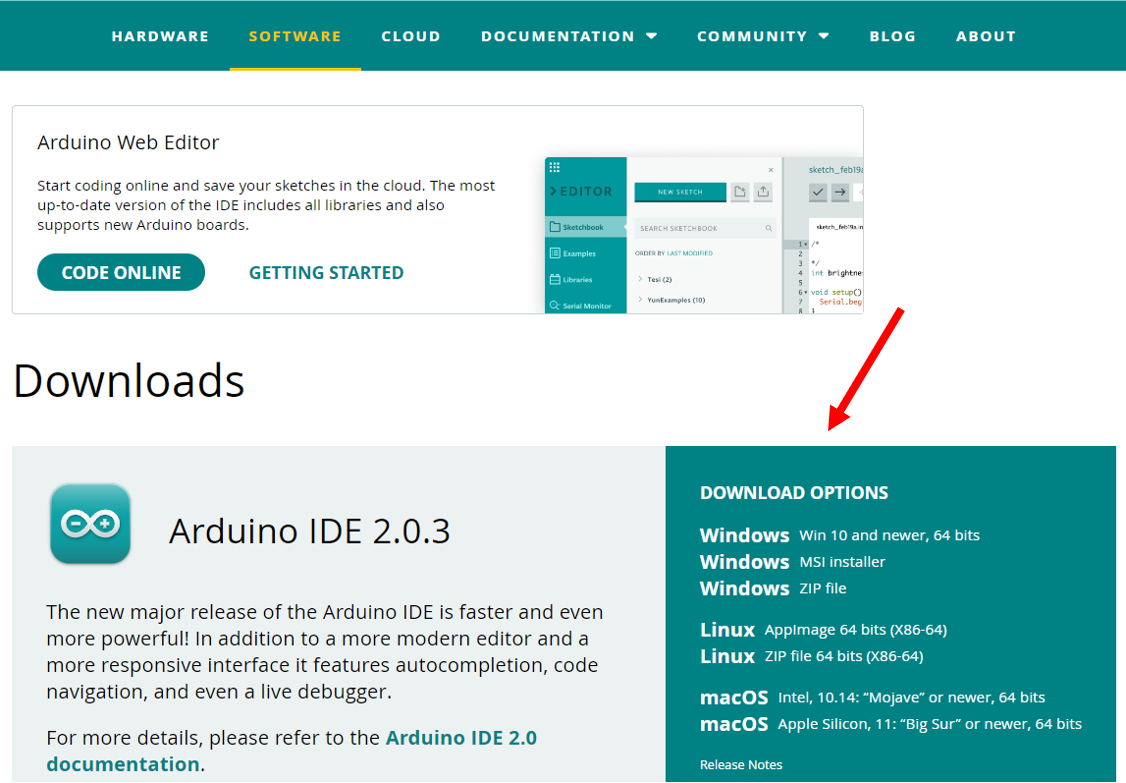
\includegraphics[width = \imageWidth]{Assets/Downloads_page.png}
        \end{center}
        
        \item Next, open the IDE and head to \textbf{File → Preferences}, and enter the following URL into the 'Additional boards manager URLs':
        \textbf{https://dl.espressif.com/dl/package\_esp32\_index.json} and hit OK.
        
        \begin{center}
            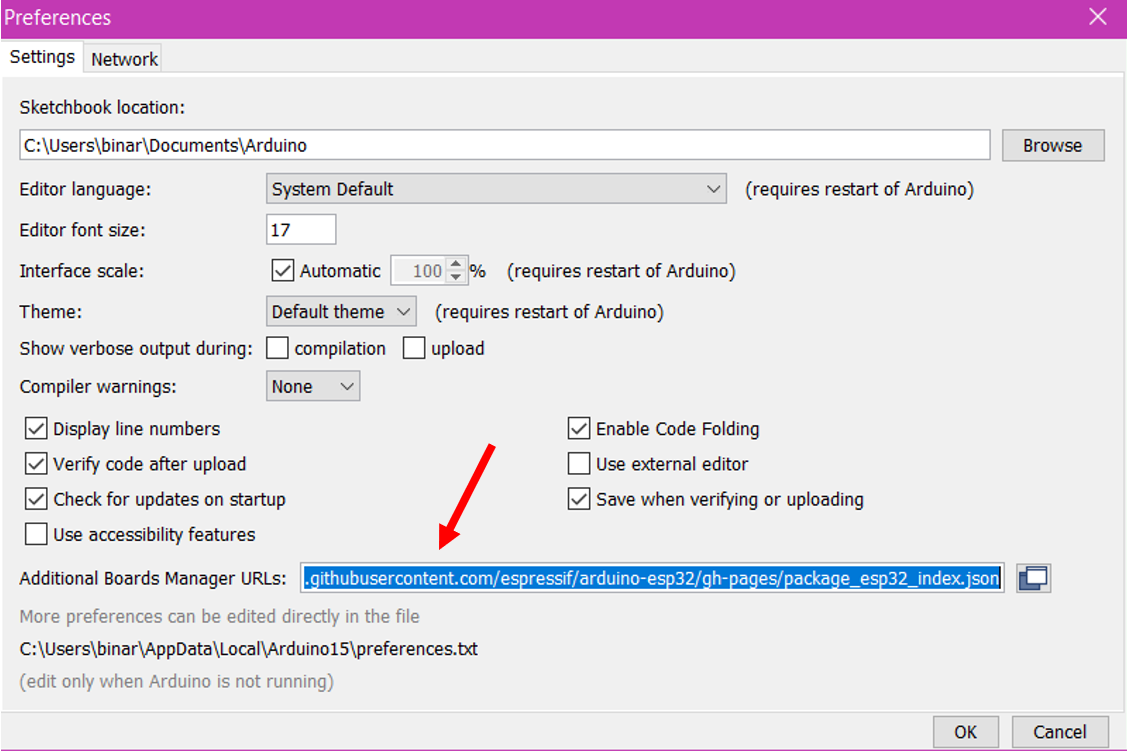
\includegraphics[width = \imageWidth]{Assets/Esp_url.png}
        \end{center}
        
        \newpage
        \item Go back to the IDE and head to \textbf{Tools → Board → Boards Manager}. In the old IDE, a new pop-up should appear, and in IDE 2, the toolbox should appear on the left hand side as shown below:
        
        \begin{center}
            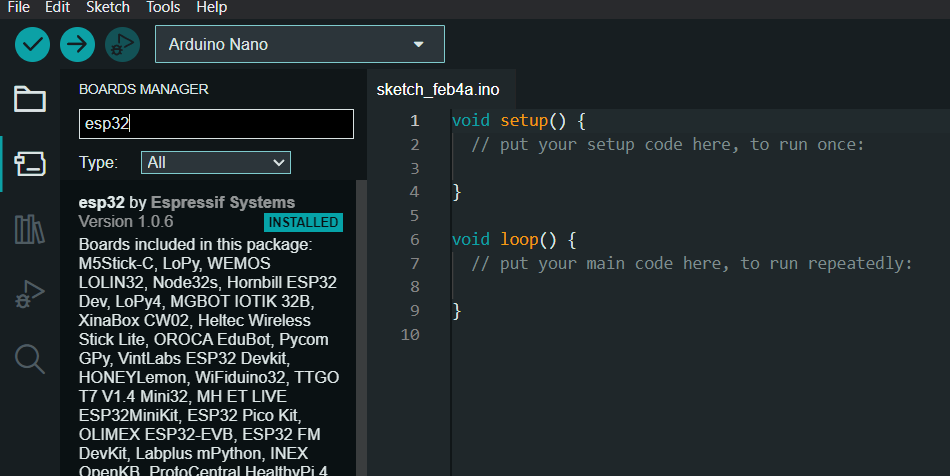
\includegraphics[width = \imageWidth]{Assets/Boards_manager.png}
        \end{center}
    
        \item To upload code to a board, plug it into the computer and make sure the board is chosen and the port specified (\textbf{Tools → Port → 'Select correct port'}). 
        Then, hit the right-facing arrow to upload. Remember to hold down the boot button on the ESP32 while uploading.
        \begin{center}
            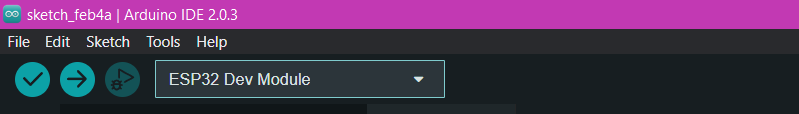
\includegraphics[width = \imageWidth]{Assets/Upload.png}
        \end{center}
        For the ESP32 uploading, once the message below is seen, release the boot button and press the reset button.
        \begin{center}
            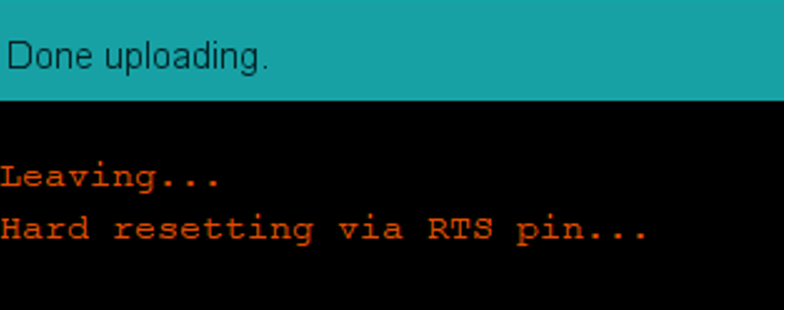
\includegraphics[scale = 0.7]{Assets/Hard_reset.png}
        \end{center}
    \end{enumerate}

\newpage
\section*{Additional Considerations for the ESP32}
    There is some additional information to be aware of when using an ESP32 with the Arduino IDE.
    \begin{enumerate}
        \item In most cases, on Windows computers, the ESP32 port is not automatically detected on the Arduino IDE. To determine which port the ESP32 is connected to, head to the Windows search bar and enter 'Device Manager'. In the device manager, click
        \newline
        'Ports (COM \& LPT)'. Under this dropdown, search for your ESP32 board COM port.
        \begin{center}
            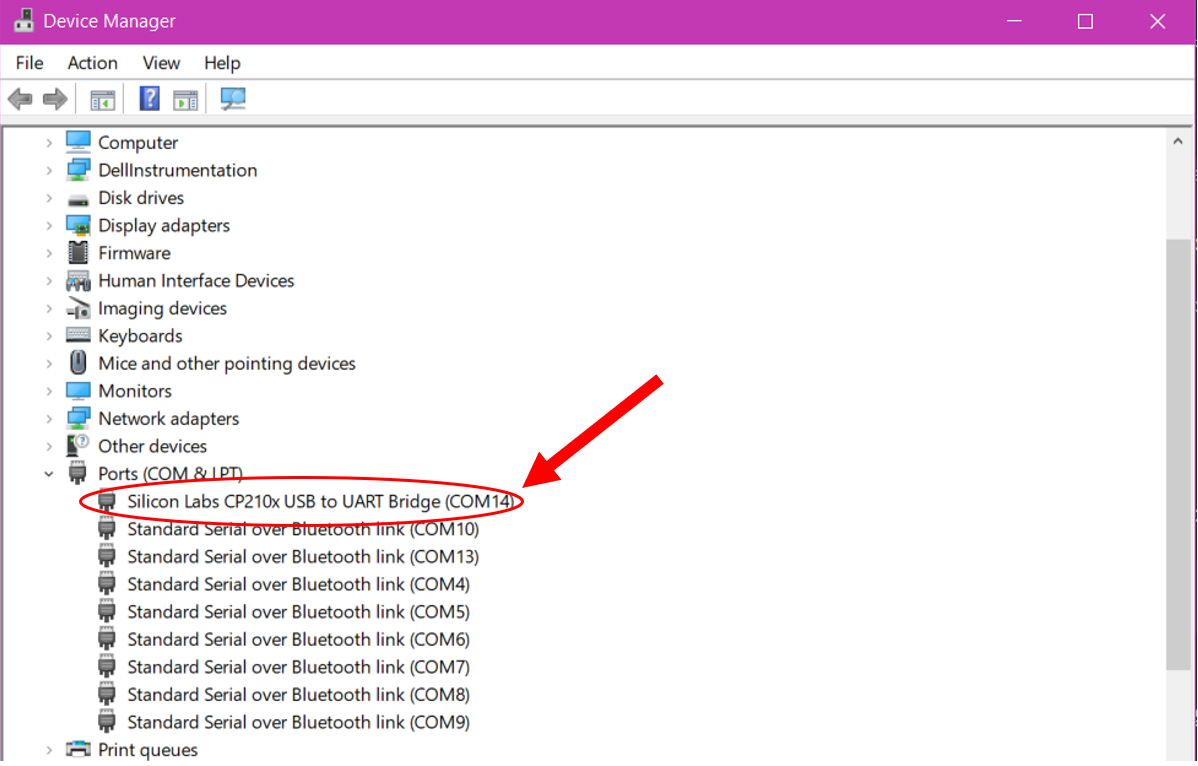
\includegraphics[width = \imageWidth]{Assets/device_manager.png}
        \end{center}
        \item If using a Windows 11 computer, an additional driver must be installed. Download our 'ESP\_DRIVER', and unzip the folder. Inside, right click on 'silabser.inf' and click 'install'.
        \begin{center}
            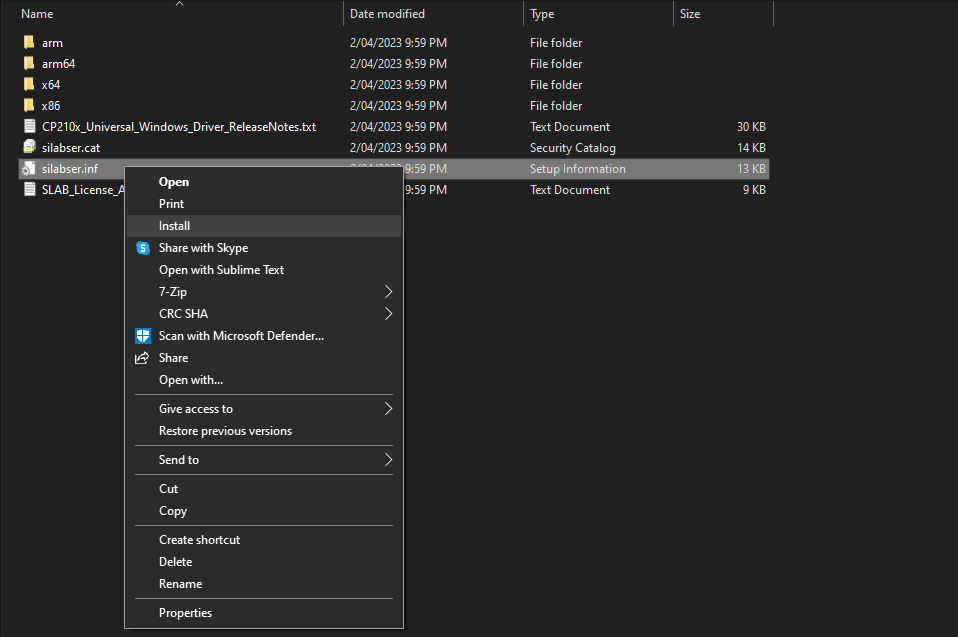
\includegraphics[width = \imageWidth]{Assets/esp_driver.png}
        \end{center}
    \end{enumerate}
\newpage
\section*{Overview of the Arduino and ESP32}
    \begin{center}
    
    Arduinos and ESPs are types of microcontrollers that can control simple to complex electronics. At a basic fundamental level, they are able to control other electrical devices, and read incoming data.
    In this tutorial, purple boxes indicate new knowledge on component or code.
    \vspace{10mm}
    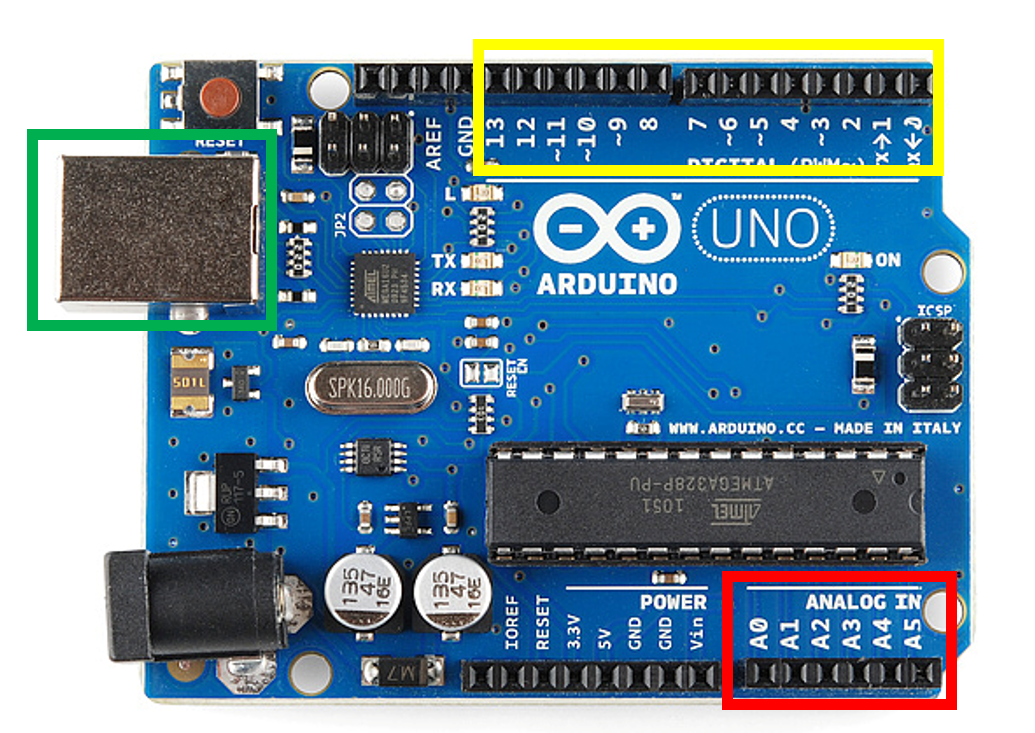
\includegraphics[scale = 0.7]{Assets/Arduino_overview.png}

    \begin{itemize}
        \item Indicated above in green, is the data cable connection for
        uploading codes from the computer. Connecting this also provides power to the board
        \item Indicated in yellow, are the digital ports. These ports are able to interpret and send signals in binary. That is, they sense or output either ON or OFF
        \begin{itemize}
            \item Note that the ports with a tilde ($\sim$) are able to give pwm outputs.
        \end{itemize}
        \item Indicated in red are the analog ports. These ports are able to interpret signals in a range. For example, they can read a range of 0 - 255.
        \begin{itemize}
            \item Note that analog ports may also be used as digital ports but not vice versa. Also, analog ports may only read in analog, they cannot write in pwm
        \end{itemize}
        \item GND - These ports are used as a negative terminal
        \item 5V/3.3V - These are the voltage supply ports
    \end{itemize}
    \end{center}

\newpage
\begin{center}
    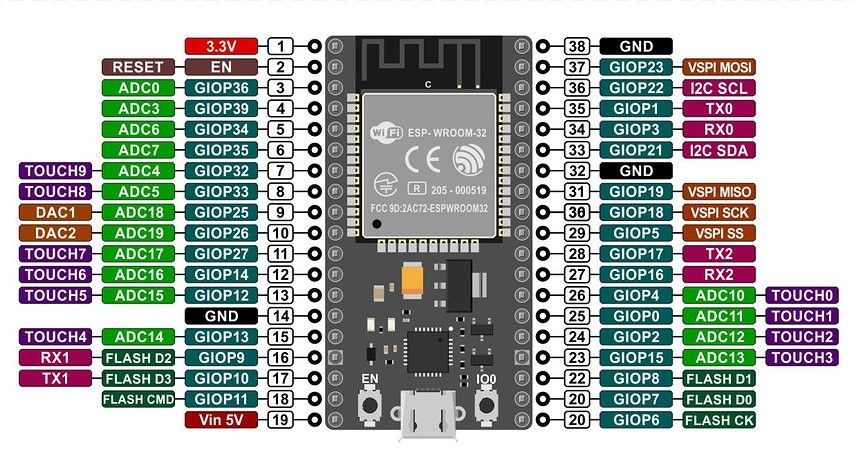
\includegraphics[scale = 2]{Assets/Esp_pinout.jpg}
    \begin{itemize}
        \item The pins in green are the GPIO pins which can serve as inputs and outputs unless otherwise signed
        \item Ports labelled ADC can be used to read analog signals
        \item Ports labelled TOUCH have internal capacitive touch sensors. For example, these pins can be used as touch sensors using just a finger
        \item All pins that can use output can use PWM
    \end{itemize}
\end{center}

\newpage
\section*{Lesson 1: Blinking an LED}
    \subsection*{What You'll Need:}
        \begin{itemize}
            \item Arduino/ESP32
            \item LED
            \item Breadboard
        \end{itemize}
        \begin{mdframed}[linewidth = 3, linecolor = turbo_purple]
        \textbf{LED:}
        \\
        The new component is a light emitting diode (LED). It is a low-current light source that operates with currents only in a single direction. The longer pin is the positive terminal.
        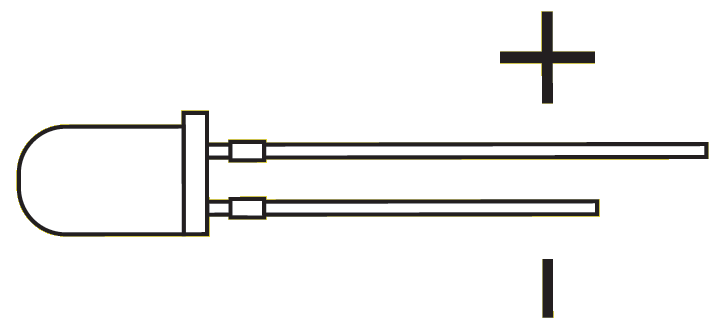
\includegraphics[scale = 0.3]{Assets/led.png}
        \end{mdframed}
    \subsection*{Wiring Diagram:}
        \begin{center}
            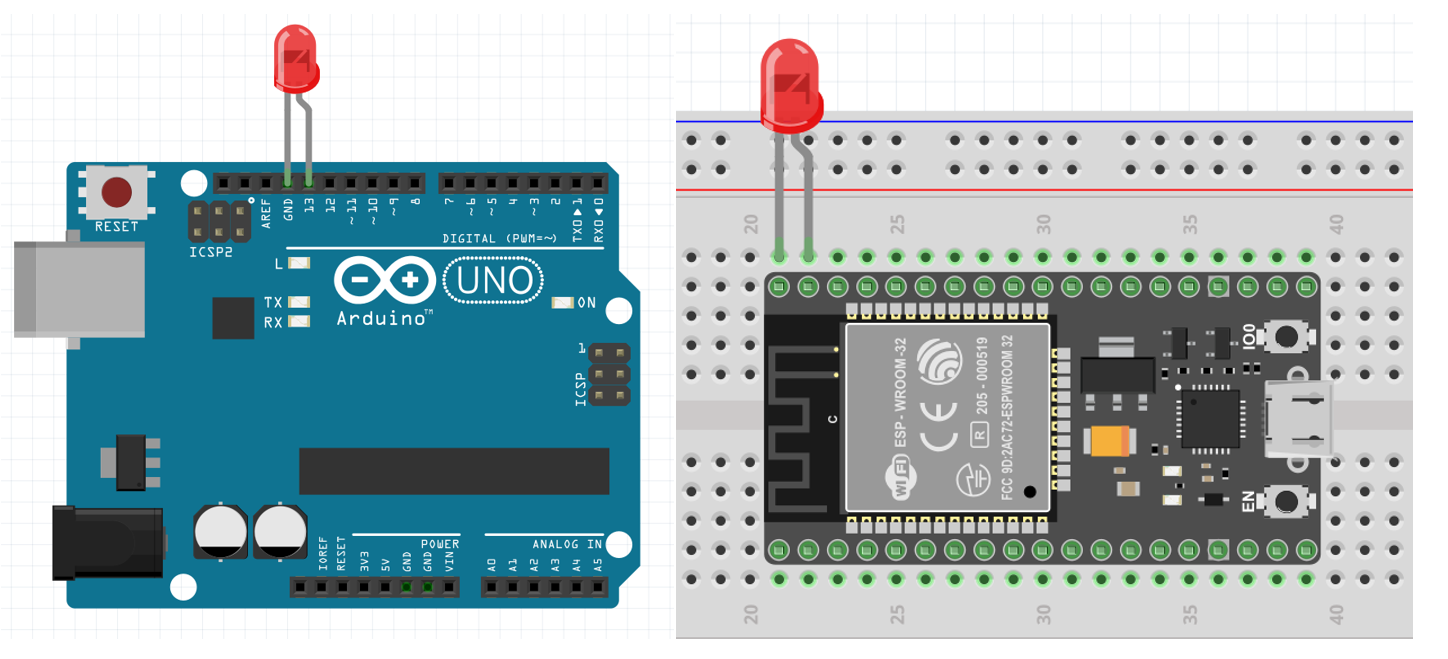
\includegraphics[width = \diagramWidth]{Assets/LED_diagram.png}
        \end{center}
   \subsection*{Directions:}
        \begin{center}
            \begin{tabularx}{\textwidth} { 
                | >{\raggedright\arraybackslash}X 
                | >{\raggedright\arraybackslash}X | }
                \hline
                \multicolumn{1}{|c|}{\textbf{Arduino}} & 
                \multicolumn{1}{|c|}{\textbf{ESP32}} \\
                \hline
                \begin{enumerate}
                    \item Plug the led with positive terminal in port 13, and negative terminal in ground
                \end{enumerate} &
                \begin{enumerate}
                    \item Plug the led with positive terminal in port G23, and negative terminal in ground
                \end{enumerate} \\
                \hline
            \end{tabularx}
        \end{center}

\newpage
\subsection*{Code (Light the LED):}
    \begin{mdframed}[linewidth = 3, linecolor = turbo_purple]
        
\includegraphics[height = \codeHeight]{Assets/int.png} \\
        This line creates a new integer variable of any name and sets it to a specified value. A variable name can be anything (note capitals are identified as different characters). A variable is a sort of container that stores information in it. \\ \\
        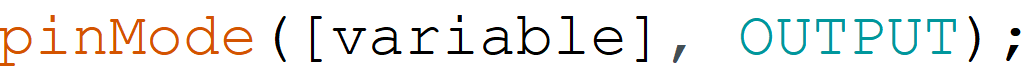
\includegraphics[height = \codeHeight]{Assets/pinmode.png} \\
        This line assigns a chosen variable as an output or an input on the Arduino. The Arduino takes the information from the variable and uses it as a port address. \\ \\
        
\includegraphics[height = \codeHeight]{Assets/dwrite.png} \\
        This line digitally powers the chosen port to either high or low,  meaning current on or off.
    \end{mdframed} 
    \vspace{20mm}
    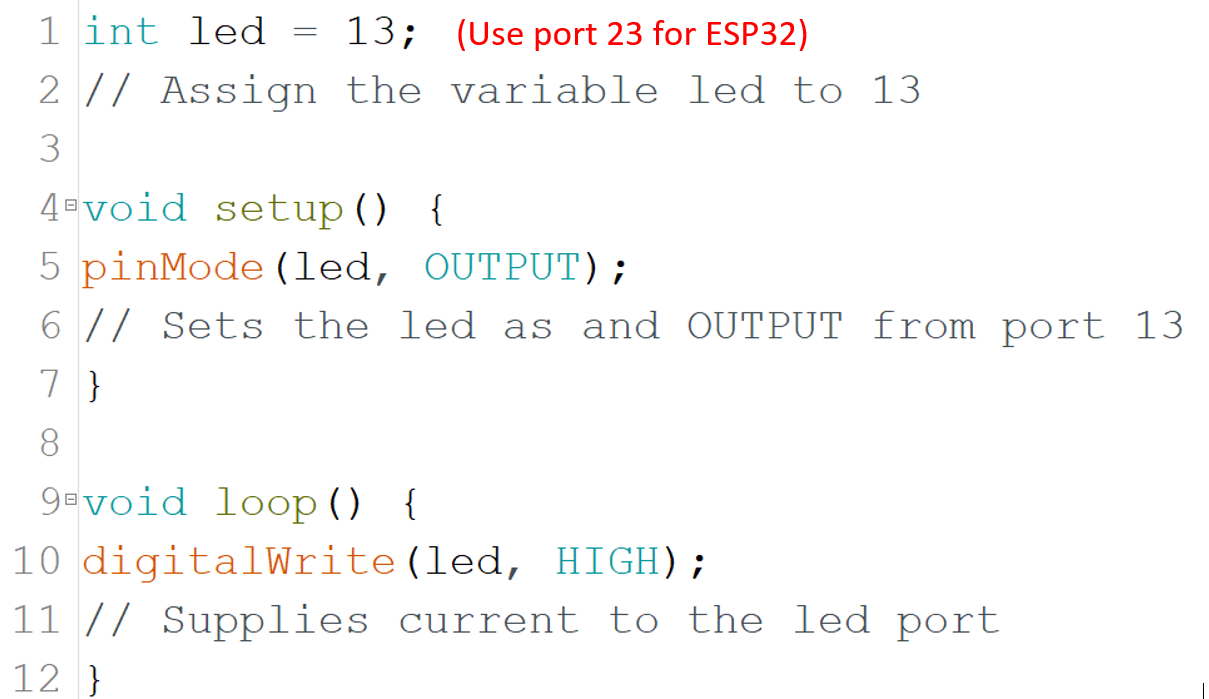
\includegraphics[width = \diagramWidth]{Assets/Light_led.png} \\
    Upload to the Arduino/ESP32 and the LED should light up.

\newpage
\subsection*{Code (Blinking the LED):}
    \begin{mdframed}[linewidth = 3, linecolor = turbo_purple]
        
\includegraphics[height = \codeHeight]{Assets/delay.png} \\
        Pauses code operation for a period of time (milliseconds). The Arduino/ESP32 will continue its previous given operations during this period.
    \end{mdframed}
    \vspace{10mm}
    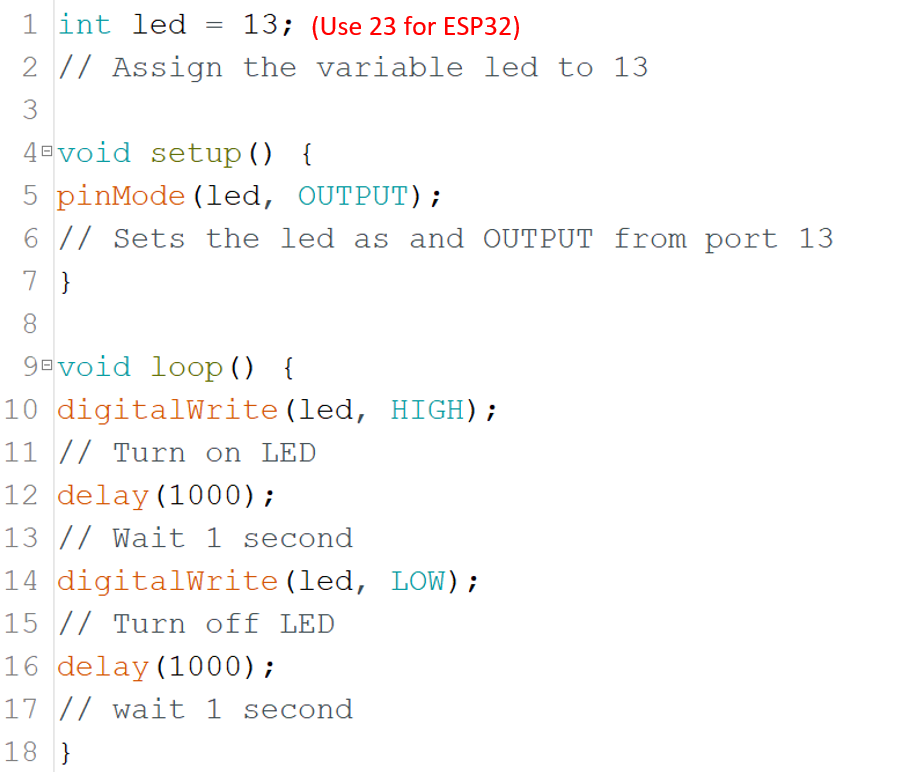
\includegraphics[width = \diagramWidth]{Assets/blink_led.png} \\
    Upload the code to the Arduino/ESP32 and the LED should blink. Changing the value of the delay will change the frequency of the blinking.

\newpage
\section*{Lesson 2: LED with a button}
    \subsection*{What You'll Need:}
        \begin{itemize}
            \item Arduino/ESP32
            \item LED
            \item Breadboard
            \item 2 wires (male to male)
            \item Button
        \end{itemize}
        \begin{mdframed}[linewidth = 3, linecolor = turbo_purple]
            \textbf{Breadboard:} \\
            A breadboard is a non-soldering technique of connecting components. Wires in the same column are connected, and some breadboards have indicated rows connected horizontally as shown below. \\
            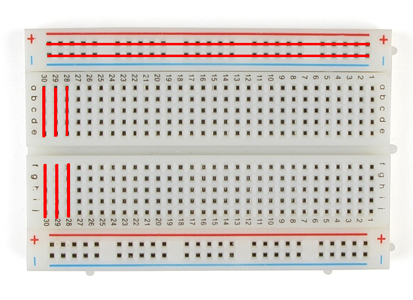
\includegraphics[scale = 0.7]{Assets/breadboard.png} \\
            \textbf{Button:} \\
            A button is a simple method of breaking a circuit. Standard buttons have 2 pins however, some buttons have 4. Indicated below, pressing a button connects 1 & 3 to 2 & 4. \\
            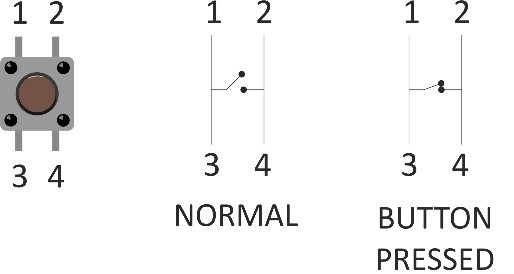
\includegraphics[scale = 1]{Assets/button.jpg}
        \end{mdframed}
\newpage
\subsection*{Wiring Diagram:}
    \begin{center}
        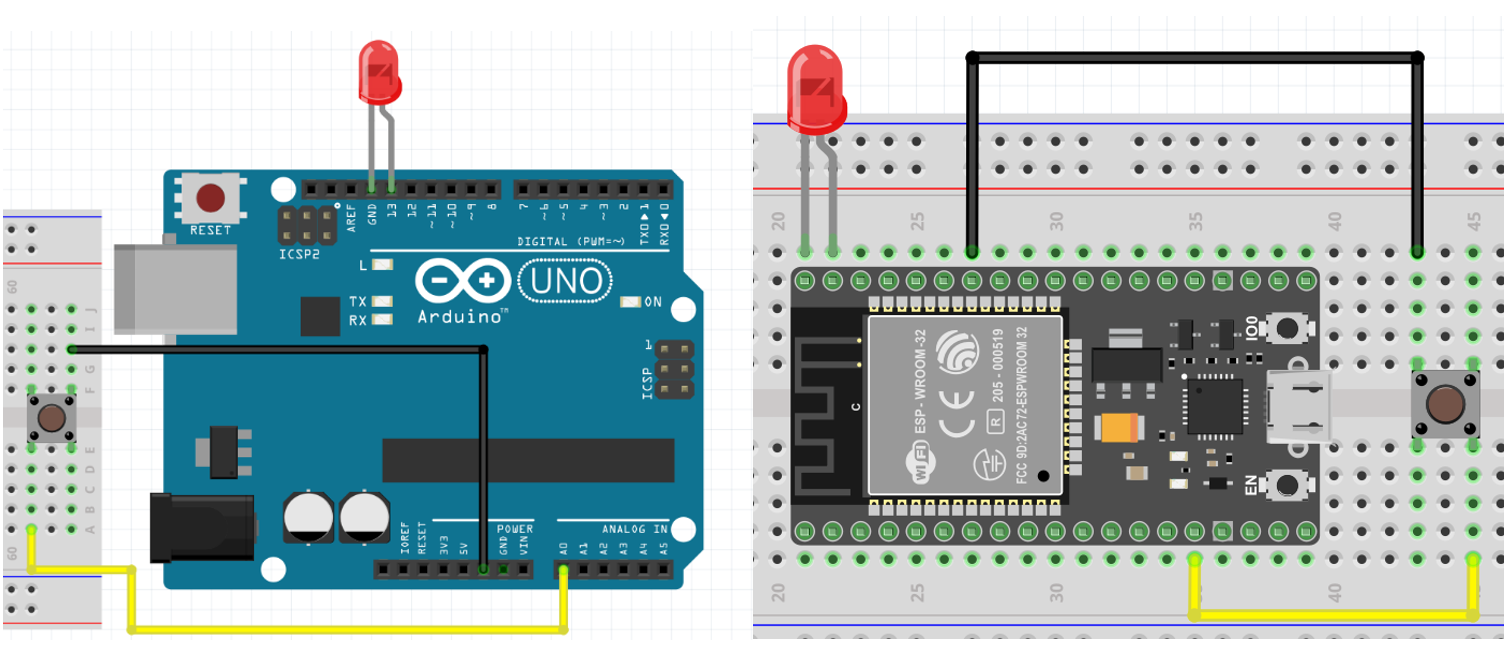
\includegraphics[width = \diagramWidth]{Assets/button_led.png}
    \end{center}

\subsection*{Directions:}
\begin{center}
    \begin{tabularx}{\textwidth} { 
        | >{\raggedright\arraybackslash}X 
        | >{\raggedright\arraybackslash}X | }
        \hline
        \multicolumn{1}{|c|}{\textbf{Arduino}} & 
        \multicolumn{1}{|c|}{\textbf{ESP32}} \\
        \hline
        \begin{enumerate}
            \item Plug the positive terminal of the Arduino in port 13, and negative to GND. Connect the button to the breadboard as indicated.
            \item Using wires, connect the top left terminal to port A0, and connect the bottom right terminal to GND
        \end{enumerate} &
        \begin{enumerate}
            \item Plug the positive terminal of the ESP32 in G23, and negative to GND. Connect the button to the breadboard as indicated.
            \item Using wires, connect the top left terminal to GND, and connect the bottom right terminal to G12
        \end{enumerate} \\
        \hline
    \end{tabularx}
\end{center}

\subsection*{Code:}
    \begin{mdframed}[linewidth = 3, linecolor = turbo_purple]
        
\includegraphics[height = \codeHeight]{Assets/dread.png} \\
        Reads the incoming digital signal from a sensor. \\
        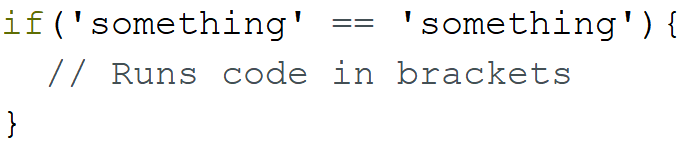
\includegraphics[height = 21mm]{Assets/if.png} \\
        Logic statements are used to give the boards intelligence. For example, if a variable is equal to a certain number, the microcontroller will run a specific command for those conditions. Operators such as the following may be used: \\
        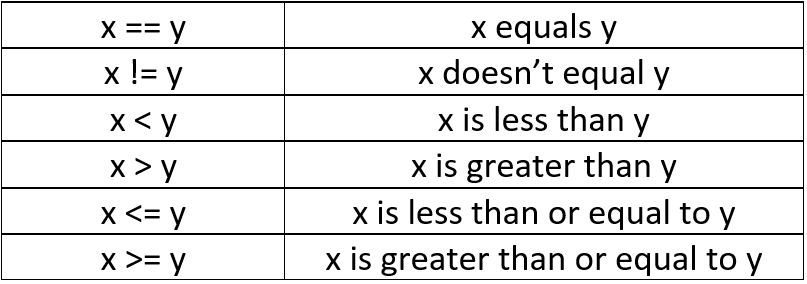
\includegraphics[scale = 0.4]{Assets/operators.png}
    \end{mdframed}
    \newpage
    \begin{center}
        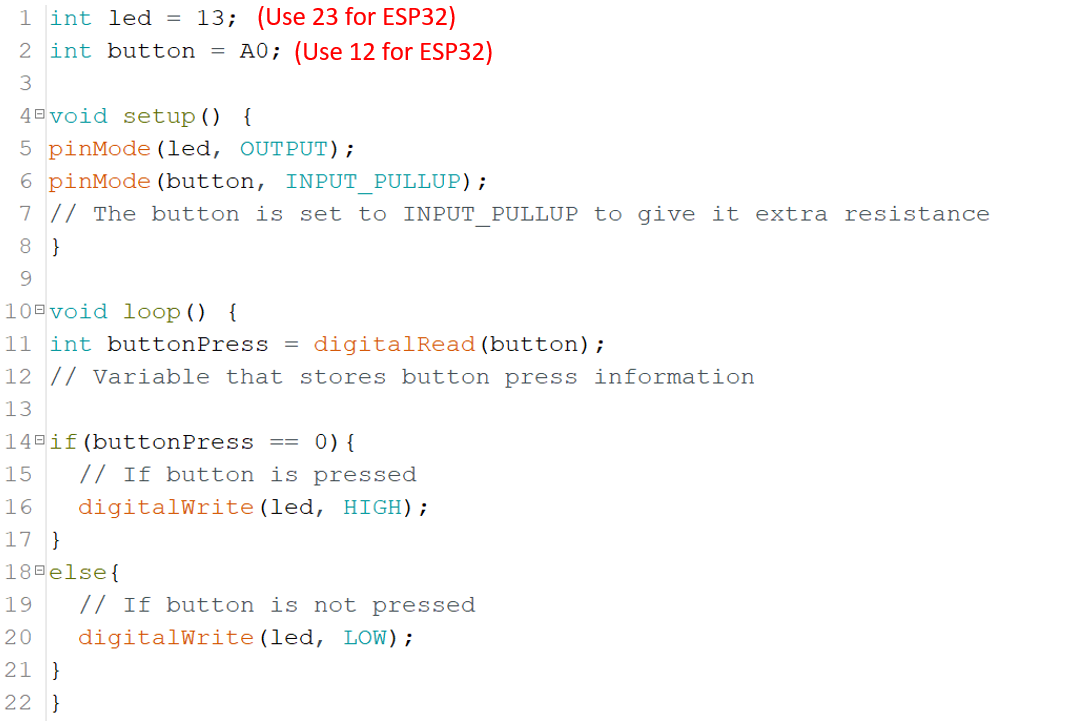
\includegraphics[width = \diagramWidth]{Assets/led_button.png}\\
    \end{center}
    Upload the code to the Arduino/ESP32. When the button is not pressed, the LED should be off, and when the button is pressed, the LED should turn on.

\newpage
\section*{Lesson 3: Dimming an LED}
    \subsection*{What You'll Need:}
            \begin{itemize}
                \item Arduino/ESP32
                \item LED
                \item Breadboard
                \item Potentiometer
                \item 5 wires (male to male)
            \end{itemize}
        \begin{mdframed}[linewidth = 3, linecolor = turbo_purple]
            \textbf{LED:}
            \\
            Potentiometers are a sort of variable resistor. They are a sensory input for the Arduino that gives a value between 0 and 1024 depending on how far the knob is twisted. Note that the signal must be used by an analog port. The VCC and GND ports are interchangeable however the signal must always be in the middle. \\
            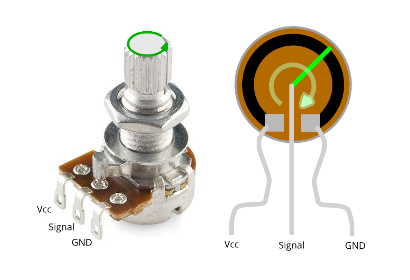
\includegraphics[scale = 1]{Assets/pot.png}
        \end{mdframed}
    \subsection*{Wiring Diagram:}
    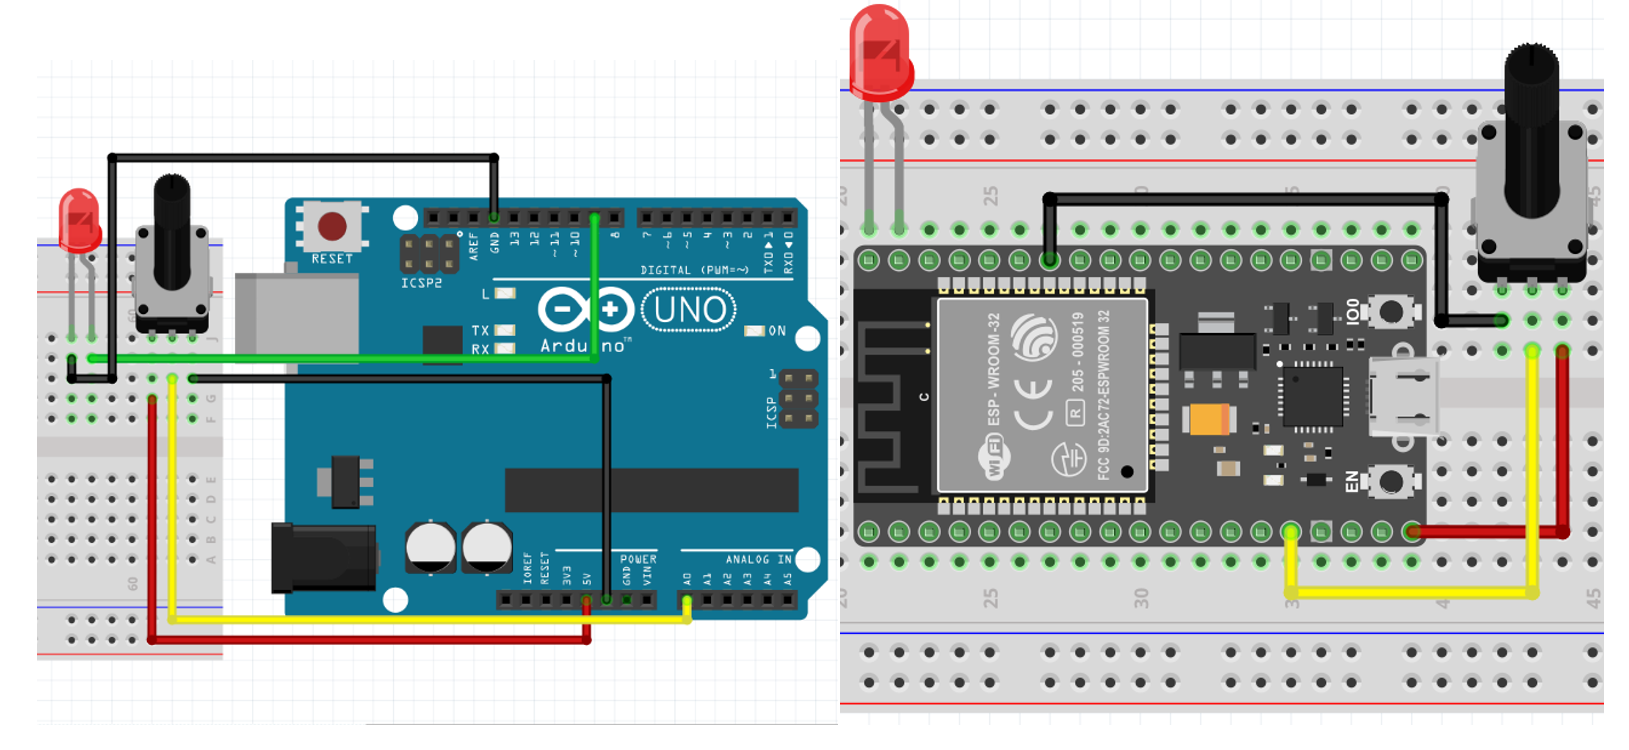
\includegraphics[width = \diagramWidth]{Assets/arduino_esp_pot.png}
\newpage
\subsection*{Directions:}
\begin{center}
    \begin{tabularx}{\textwidth} { 
        | >{\raggedright\arraybackslash}X 
        | >{\raggedright\arraybackslash}X | }
        \hline
        \multicolumn{1}{|c|}{\textbf{Arduino}} & 
        \multicolumn{1}{|c|}{\textbf{ESP32}} \\
        \hline
        \begin{enumerate}
            \item Plug in the LED and potentiometer into the breadboard.
            \item Connect a GND wire to the right side of the potentiometer and a 5V wire to the left side
            \item Connect a wire from port A0 to the middle pin on the potentiometer
            \item Connect a GND wire and a wire from port 9 correctly to the LED
        \end{enumerate} &
        \begin{enumerate}
            \item Plug in the LED to port G23 and plug the potentiometer into the breadboard
            \item Connect a GND wire to the left side of the potentiometer and a 5V wire to the right side
            \item Connect a wire from port G12 to the middle pin on the potentiometer
        \end{enumerate} \\
        \hline
    \end{tabularx}
\end{center}
\subsection*{Code (Serial Feedback):}
    \begin{mdframed}[linewidth = 3, linecolor = turbo_purple]
        
\includegraphics[height = \codeHeight]{Assets/begin.png} \\
         Starts serial communication with the computer \\ \\
         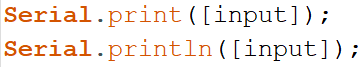
\includegraphics[height = 14mm]{Assets/serial.png} \\ 
         Displays the specified input to the monitor. Using ‘println’ creates a new line of text.
    \end{mdframed}

\newpage
    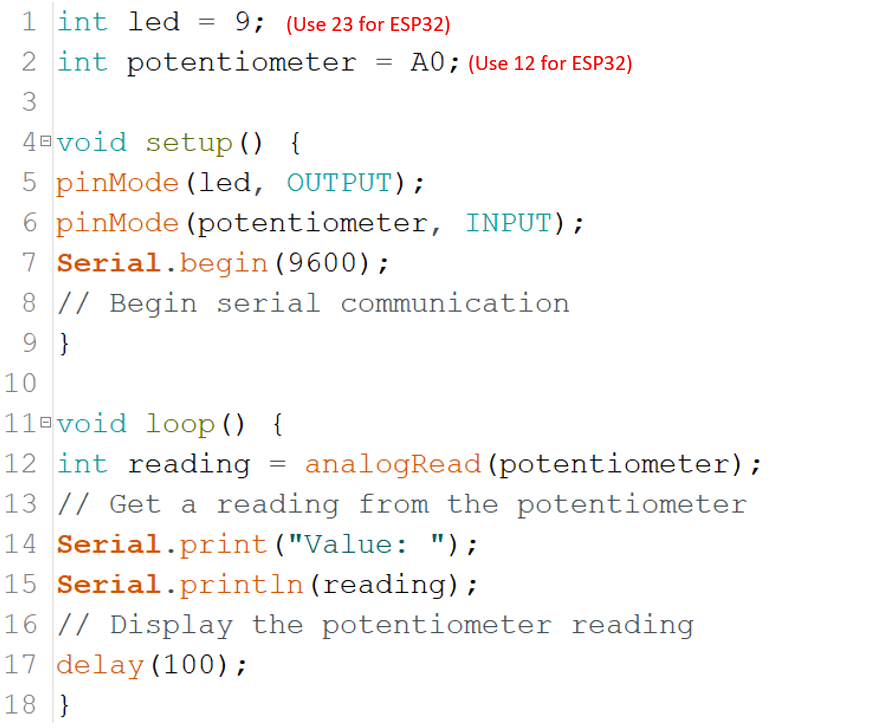
\includegraphics[width = \diagramWidth]{Assets/serial_code.png} \\
    Upload the code to the Arduino/ESP32 and open the serial monitor in the top right corner (red arrow). The values should resemble the following. Twist the potentiometer to change the value. \\
    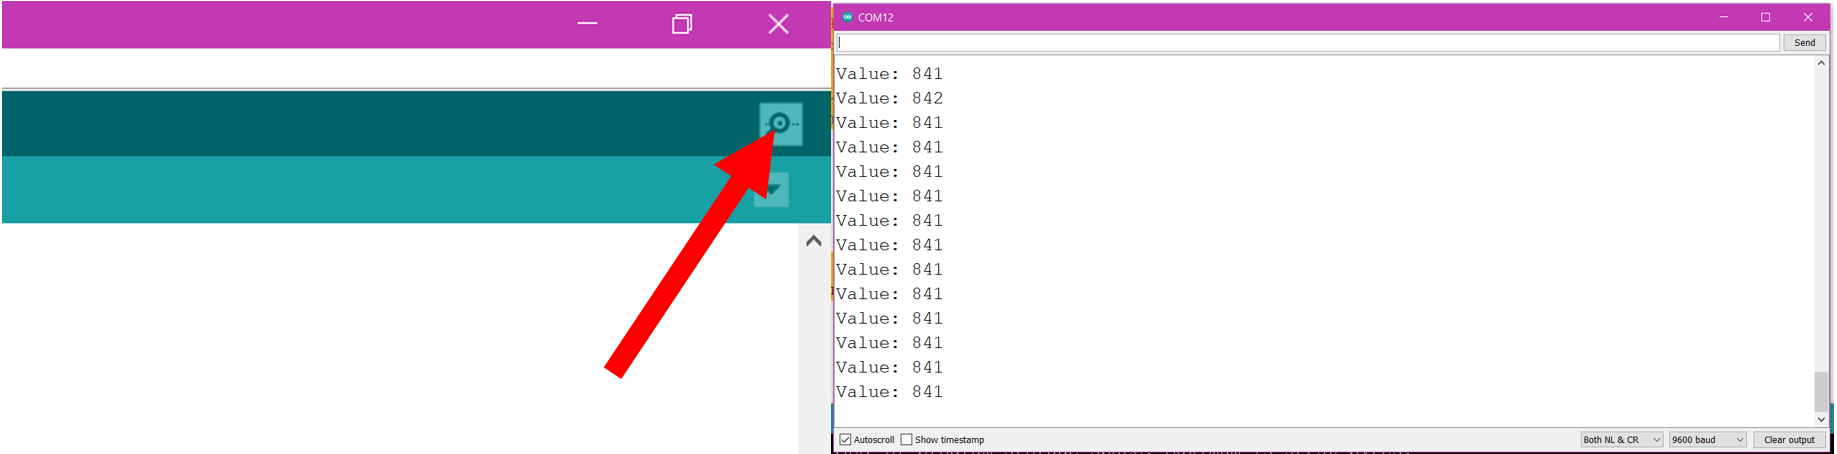
\includegraphics[width = \diagramWidth]{Assets/serial_monitor.png}

\newpage
\subsection*{Code (Dimming LED Arduino):}
    \begin{mdframed}[linewidth = 3, linecolor = turbo_purple]
        
\includegraphics[height = \codeHeight]{Assets/aread.png} \\
         This line reads for an incoming analog information (range of numbers) from a port. \\
         
\includegraphics[height = 8mm]{Assets/awrite.png} \\ 
         This line sends a power value between 0 and 255 to the specified port. This line can be used to send a range of powers. \\
         
\includegraphics[height = 6mm]{Assets/map.png} \\
         The map function takes in a value and checking its position in the larger range, rewrites its position in a lower range. After the number, the first two numbers are upper and lower bounds of the incoming number range (numbers above are only examples). The second two numbers are the output bounds. Visualisation for this example is shown below. \\
         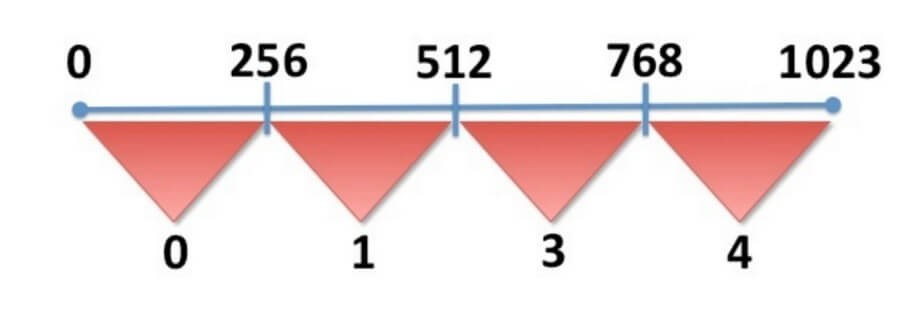
\includegraphics[scale = 0.3]{Assets/map_diagram.jpg}
    \end{mdframed}
    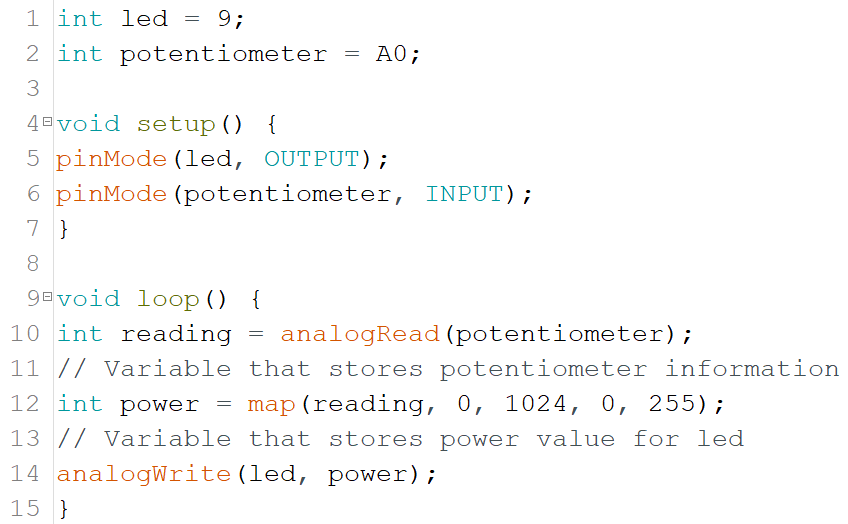
\includegraphics[width = \diagramWidth]{Assets/arduino_pot.png} \\
    Upload the code to the Arduino and the LED should brighten when the knob is twisted.

\newpage
\subsection*{Code (Dimming LED ESP32):}
    \begin{mdframed}[linewidth = 3, linecolor = turbo_purple]
        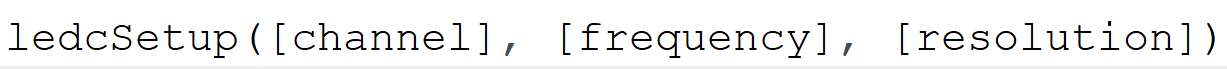
\includegraphics[height = 8mm]{Assets/ledcsetup.png} \\
         This line is used to set up the properties of the PWM signal, and the channel it will run on. Resolution is how many bits are used for the signal (up to 16 bits). The ESP32 has 16 PWM channels and any GPIO can be used to output PWM using a channel. \\
         
\includegraphics[height = 8mm]{Assets/ledcattach.png} \\ 
         This line is used to assign a GPIO pin to a PWM channel. This will be where your PWM channel will output its signal. \\
         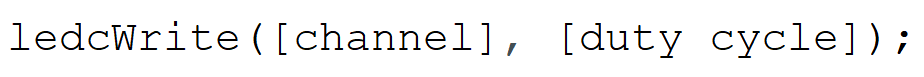
\includegraphics[height = 8mm]{Assets/ledcwrite.png} \\ 
         This function is essentially the same as the analogWrite() function. It’s used to write the duty cycle to the channel. The duty cycle takes a value between 0 and 100.  \\
    \end{mdframed}
    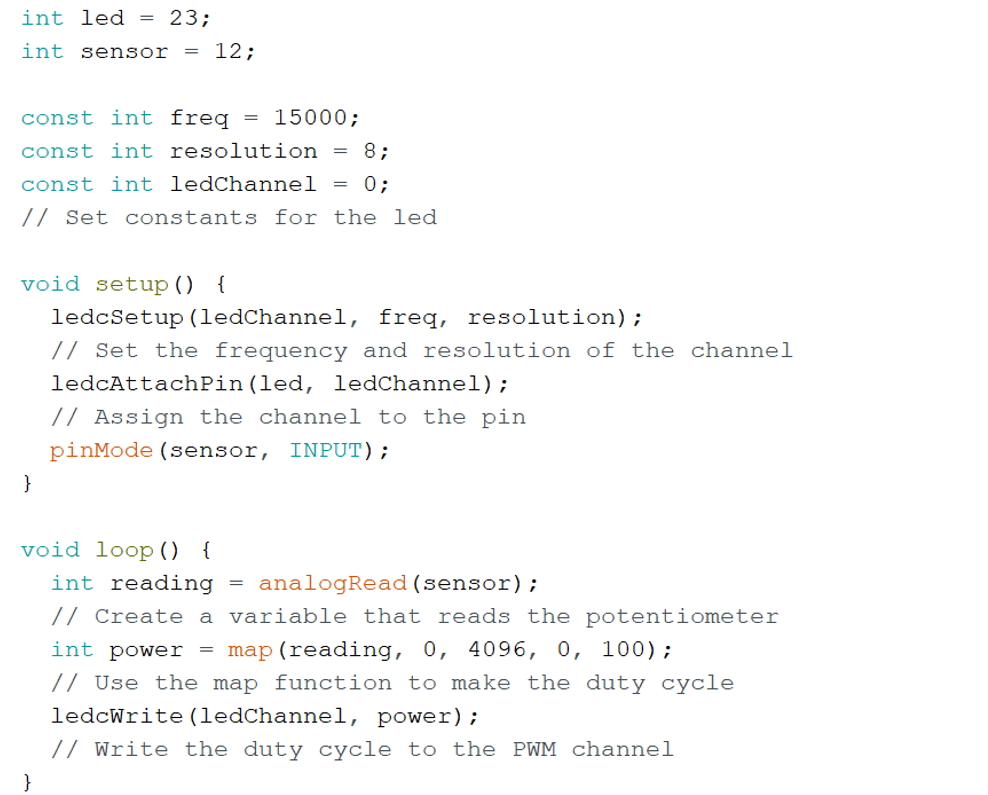
\includegraphics[width = \diagramWidth]{Assets/esp_pot.png} \\
    Upload the code to the ESP32 and the LED should brighten as the potentiometer is twisted. 

\newpage
\section*{Lesson 4: Ultrasonic Sensor}
    \subsection*{What You'll Need:}
        \begin{itemize}
            \item Arduino/ESP32
            \item Ultrasonic Sensor (HC-SR04)
            \item 4 wires (male to female) (Arduino)
            \item 4 wires (female to female) (ESP32)
        \end{itemize}
        \begin{mdframed}[linewidth = 3, linecolor = turbo_purple]
            \textbf{Ultrasonic Sensor:} \\
            The HC-SR04 ultrasonic sensor sends out a sound and measures the time taken for the to return. It uses this technique to measure distances from objects. Note it has difficulty sensing objects that absorb sound like foam. Though the ultrasonic gives a range of readings, digital ports may be used to read it. \\
            \includegraphics[scale = 0.3]{Assets/Ultrasonic.jpg}
        \end{mdframed}
    \subsection*{Wiring Diagram:}
        \includegraphics[width = \diagramWidth]{Assets/arduino_esp_ultrasonic.png}

\newpage
    \subsection*{Directions:}
        \begin{center}
            \begin{tabularx}{\textwidth} { 
                | >{\raggedright\arraybackslash}X 
                | >{\raggedright\arraybackslash}X | }
                \hline
                \multicolumn{1}{|c|}{\textbf{Arduino}} & 
                \multicolumn{1}{|c|}{\textbf{ESP32}} \\
                \hline
                \begin{enumerate}
                    \item Connect the VCC to 5V and GND to GND. Connect the Trig pin to port 12, and connect the Echo pin to port 13
                \end{enumerate} &
                \begin{enumerate}
                    \item Connect the VCC to V5 and GND to GND. Connect the Trig pin to port 23, and connect the Echo pin to port 22.
                \end{enumerate} \\
                \hline
            \end{tabularx}
        \end{center}
    \subsection*{Code:}
        \begin{mdframed}[linewidth = 3, linecolor = turbo_purple]
            \includegraphics[height = \codeHeight]{Assets/include_u.png} \\
            This is to introduce an ultrasonic library that does not come default with the software. It must be additionally downloaded. To do this, navigate to Tools -> Manage Libraries. In manage libraries, search for ultrasonic, and scroll to locate the indicated library. Once located, click install. When complete, restart the IDE, and the library should be in your Include Library as Ultrasonic. \\
            \begin{center}
                \includegraphics[width = \diagramWidth]{Assets/ultrasonic_library.png}
            \end{center}
            \includegraphics[height = 6mm]{Assets/ultrasonic_init.png} \\
            This line creates an ultrasonic object. Type in the ports of the ultrasonic as indicated by Trig and Echo. \\
            \includegraphics[height = 6mm]{Assets/ultrasonic_read.png} \\
            This returns the value currently being read by the sensor.
        \end{mdframed}
    \newpage
    \includegraphics[width = \diagramWidth]{Assets/ultrasonic_code.png} \\
    \includegraphics[width = \diagramWidth]{Assets/ultrasonic_monitor.png} \\
    Upload the code to the Arduino/ESP32 and open the Serial Monitor. The ultrasonic should be reading values as seen in the above Serial Monitor.
\newpage
\section*{Credits}
\begin{itemize}
    \item Binara Wasala
    \begin{itemize}
        \item 'Required Software' section
        \item 'Additional Considerations for the ESP32' section
        \item 'Overview of the Arduino and ESP32' section
        \item 'Lesson 1: Blinking an LED' section
        \item 'Lesson 2: LED with a button' section
        \item 'Lesson 3: Dimming and LED' section
        \item 'Lesson 4: Ultrasonic Sensor' section
    \end{itemize}
\end{itemize}
\end{document}
